\documentclass[12pt, handout=show,notes=show]{beamer}
\usetheme[width=0cm]{Goettingen}
\usecolortheme{rose}
\useoutertheme{default}
\setbeamerfont{caption}{size=\scriptsize}

\addtobeamertemplate{navigation symbols}{}{%
	\usebeamerfont{footline}%
	\usebeamercolor[fg]{footline}%
	\hspace{1em}%
	$\dfrac{\insertframenumber}{\inserttotalframenumber}$
}

\usepackage{hyperref}
\usepackage{fontspec} 
\setsansfont{Futura LT}
%\setmonofont[Scale=0.8]{Monaco} 


\usepackage{arydshln}

%\usefonttheme{serif}
%%%%lualatex on

%\usepackage{fontspec}
%%\setmainfont{EBGaramond12-Regular.otf}[
%%    SlantedFont = EBGaramond12-Regular.otf ,
%%    SlantedFeatures = {FakeSlant} ,
%%    ItalicFont  = EBGaramond12-Italic.otf ,
%%]
\usepackage{amsmath}
%Ligatures={Contextual, Common, Historical, Rare, Discretionary}
%\setmainfont[Mapping=tex-text]{Linux Libertine O}

\usepackage{mathptmx}
\usepackage{latexsym}
\usepackage{mathtools}
\usepackage{multirow}
\usepackage{caption}


\DeclarePairedDelimiter\abs{\lvert}{\rvert}%
\DeclarePairedDelimiter\norm{\lVert}{\rVert}%


\makeatletter
\let\oldabs\abs
\def\abs{\@ifstar{\oldabs}{\oldabs*}}
\let\oldnorm\norm
\def\norm{\@ifstar{\oldnorm}{\oldnorm*}}
\makeatother

\title{
	Winter Simulation Conference:\\
	Co-evolution of trade and culture.
}

\institute{8th December 2016}

\author{Simon Carrignon, Jean-Marc Montanier \& Xavier Rubio-Campillo}

\date{
	\scriptsize
	\begin{columns}
		\begin{column}{.3\textwidth}
			\begin{center}
				Barcelona Supercomputing Center	\\
				
\includegraphics[height=1cm]{images/bscLogo.jpg} \hspace{2cm}
			\end{center}
		\end{column}
		\begin{column}{.3\textwidth}
			\begin{center}
				Univ. Pompeu Fabra Complex System Lab.\\
				
\includegraphics[height=1cm]{images/upfLogo.jpeg} %declare logo image with an alias here 
			\end{center}
		\end{column}
	\end{columns}

}
\begin{document}
\begin{frame}
	\maketitle

\end{frame}

\begin{frame}{Plan of the presentation}
	\begin{enumerate}
		\item Introduction
			\vfill
		\item Model Description
			\vfill
		\item Case Study: Rome
			\vfill
	\end{enumerate}
	
\end{frame}

\section{Introduction}
\begin{frame}{Cultural Evolution}
	\begin{center}
		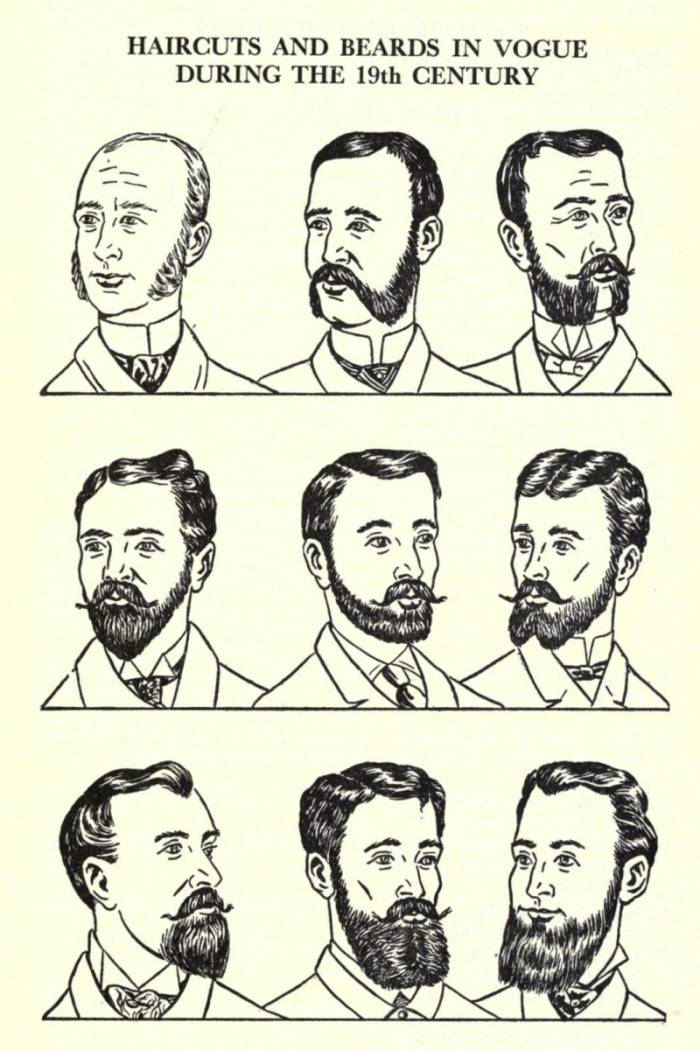
\includegraphics[width=.4\textwidth]{images/beardevo.jpg} 
	\end{center}
	How Cultural Traits Evolve?
\end{frame}

\begin{frame}{Cultural Evolution}
	\begin{center}
		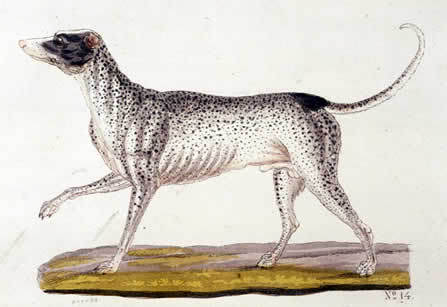
\includegraphics[width=4cm]{images/dalmatian.jpg} \hspace{2cm}
		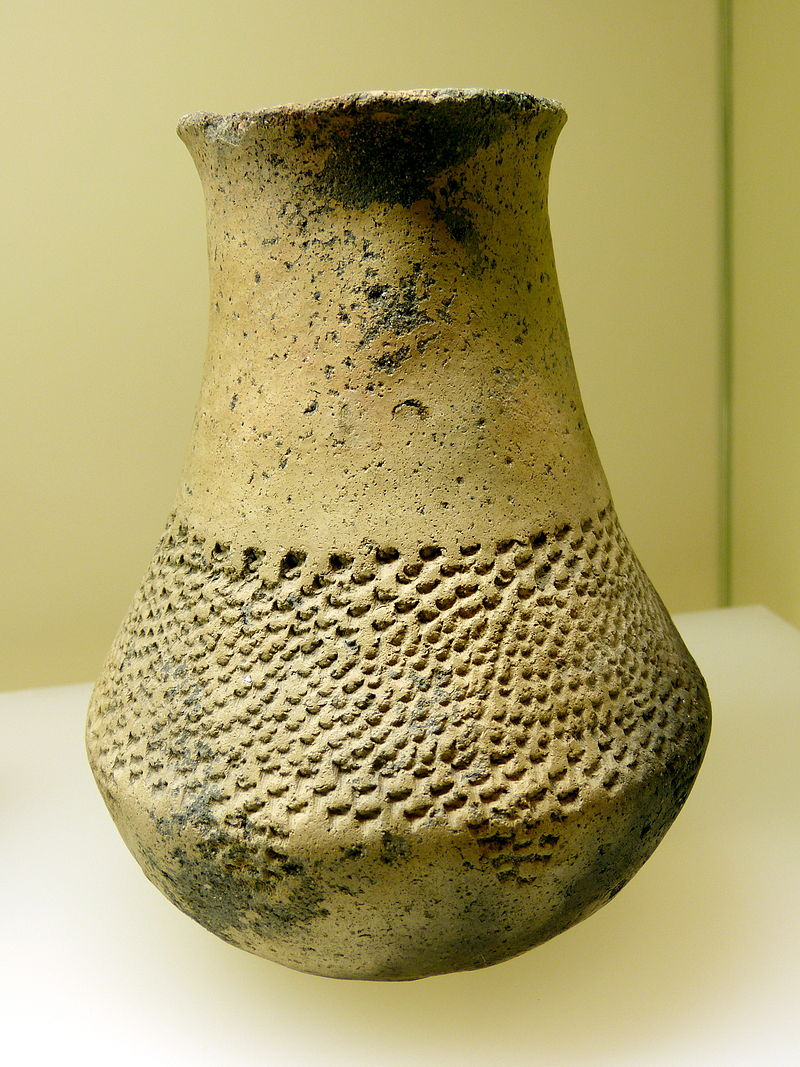
\includegraphics[width=2cm]{images/pottery.jpg}\\
		\vspace{1cm}
		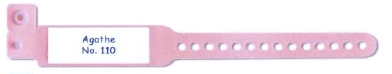
\includegraphics[width=4cm]{images/name.jpg}
	\end{center}
	Similar variants distributions
	\begin{figure}
		\begin{columns}
			\begin{column}{.8\textwidth}
				\centering
				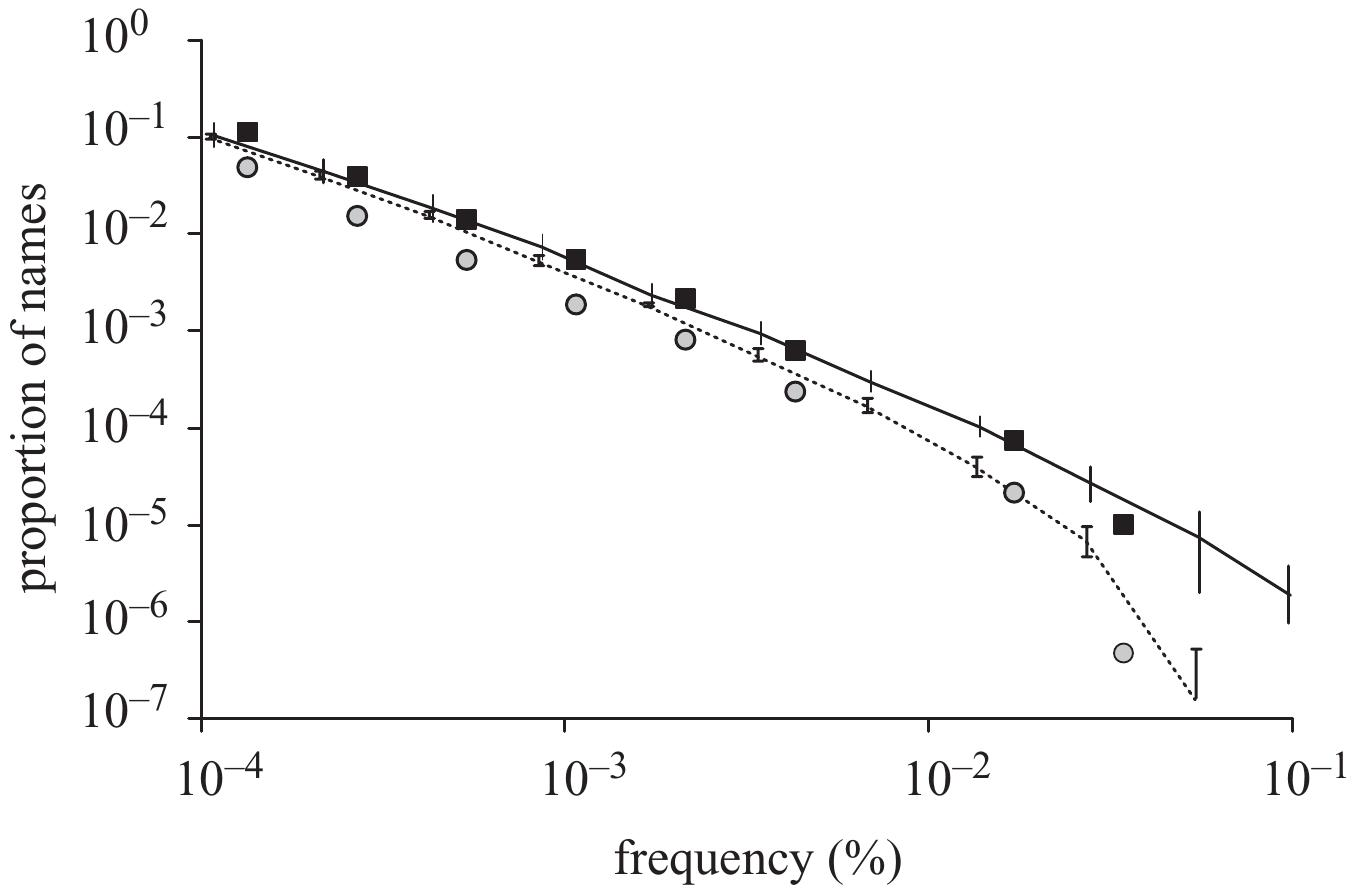
\includegraphics[width=.6\textwidth]{images/powerlawrepartition.jpg}
			\end{column}
			\begin{column}{.3\textwidth}
				\tiny
				Square: male names\\
				Circle: female names\\
			From Bentley et al,~2004.
			\end{column}
		\end{columns}
	\end{figure}
\end{frame}

\begin{frame}{What Generate Those Cultural changes?}
	Simple mechanisms (Bentley et al, 2004):
	\begin{itemize}
		\item Random Copy 
		\item Frequency biased (conformist/anti-conformist\dots)
		\item \dots	
	\end{itemize}
	\begin{figure}
		\begin{columns}
			\begin{column}{.8\textwidth}
				\centering
				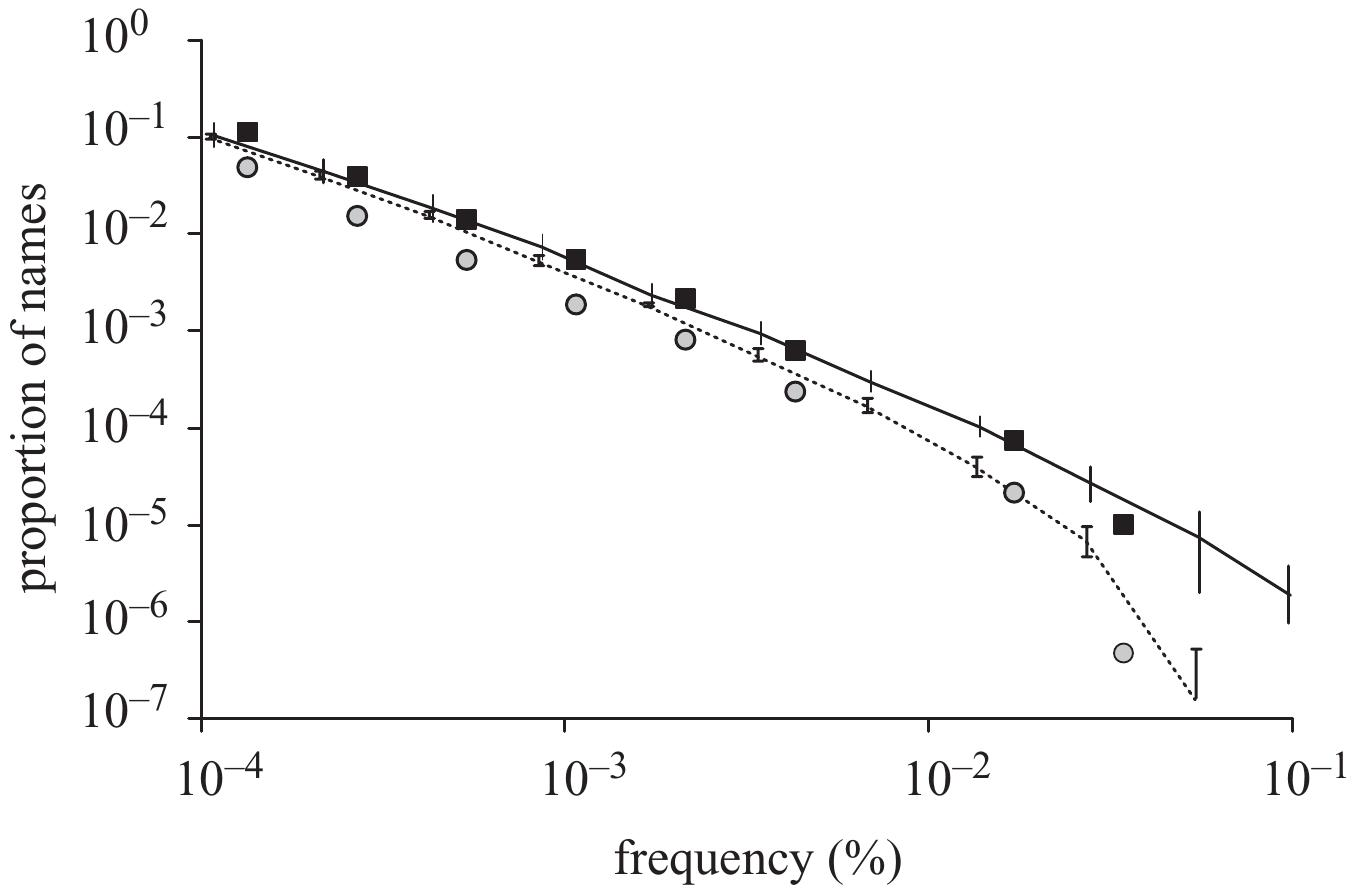
\includegraphics[width=.6\textwidth]{images/powerlawrepartition.jpg}
			\end{column}
			\begin{column}{.3\textwidth}
				\tiny
				Square: male names\\
				Circle: female names\\
				Dotted and plain lines: model result with different copy probabilities.\\
			From Bentley et al,~2004.
			\end{column}
		\end{columns}
	\end{figure}
\end{frame}

\section{Context}


\begin{frame}
	\begin{center}
		What happen when such mechanisms act on traits impacting economy?
	\end{center}
	\begin{columns}
		\begin{column}{.3\textwidth}
			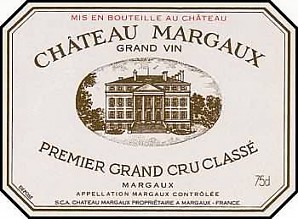
\includegraphics[width=\textwidth]{images/bordeaux.jpg}	
		\end{column}
		\begin{column}{.2\textwidth}
		\end{column}
		\begin{column}{.3\textwidth}
			
\includegraphics[width=3cm]{images/napa}	
		\end{column}
	\end{columns}
\end{frame}

\begin{frame}{Co-evolution of Economy and Culture}

	%How Simple Cultural Dynamics influence Economy That in turn will influence cultural dynamics.

	\begin{alertblock}{Interaction between Culture and Economy}
	    \begin{center}
		Cultural mechanisms transom Economy \\
		\begin{center}
		    $  \scalebox{3}{\circlearrowright}$
		\end{center}
		Economy influences Culture
	    \end{center}
	\end{alertblock}


\end{frame}

\section{ABM Framework}

\begin{frame}{A General Agent Based Framework }
	\begin{center}
	    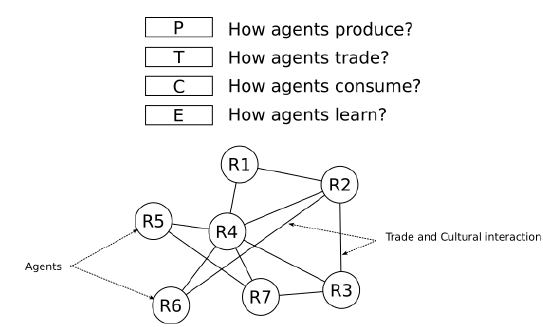
\includegraphics[width=.6\textwidth]{images/schema_model.png}
	\end{center}
\end{frame}



\begin{frame}{A General Agent Based Framework }

     Two main components:
     \vfill
    \begin{enumerate}
	\item Economic side: Bartering Economy (Gintis 2009),
		\vspace{1cm}
	\item Cultural side: ``copy the most successful'' (Bentley 2006).
    \end{enumerate}
\end{frame}
	
\begin{frame}{The Model}
	\begin{block}{1. The Economy \& the Barter Mechanism}
	    \begin{itemize}
		    \item $N$ goods
		\item $M$ Agent 
		    $\left\{
			\begin{tabular}{@{}l@{}}
			    a quantity of each Goods \\
			    $N$ values attributed to each goods\\
			\end{tabular}
			\right.$
		    \item Agents \emph{produce} one good and \emph{exchange} it to obtain the other goods.
		    \item After the exchange, the agents \emph{consume} all goods 
		\end{itemize}

	\end{block}
\end{frame}

\begin{frame}{The Model}
	\begin{block}{2. Cultural Mechanisms}
	    Every step:
	    \begin{itemize}
		    \item Economic activity (cf. previous slide).
		    \item A \emph{score} is given following $f(q_n)$  a shared \& fixed ``utility function''.
	    \end{itemize}
		After 10 steps:
		\begin{itemize}
		    \item Less successful agents \emph{copy} the most successful (Biased-Copy).
		    \item Given a probability $\mu$ the value attributed to some goods is modified (Innovation/Mutation)
		\end{itemize}
	\end{block}
\end{frame}

\begin{frame}{Experiments}
	\centering
	\textbf{Trade Model} \\Trade Mechanism + Success Biased Copy\\
	\vfill
	vs\\
	\vfill
	\textbf{Neutral Model}\\ Trade Mechanism + Random Copy\\
	 

\end{frame}


\section{Results}

\begin{frame}{Results: Random copy vs Success Biased Copy :}
    Evolution of Score
    \begin{figure}[!h]
	\centering
	\begin{tabular}{ c c}
	    Neutral Model & Trading Model \\
	    \includegraphics[width=4cm]{../img/ScoreEvolutionForRandom-G3N500.pdf}
	    & \includegraphics[width=5cm]{../img/ScoreEvolutionForTrade-G3N500.pdf}

	\end{tabular}
	\caption{Evolution of the score within the two different models for two typical run with 500 agents and 3 goods evolving during 10000 timestep.}%%
	\label{fig:scoreEvol}
    \end{figure}
\end{frame}
    


\begin{frame}{Results: Economic Dynamics}
	\begin{figure}
	    \caption{Example for 3 goods and 500 agents}
	    \begin{columns}
		\column{.5\textwidth}
		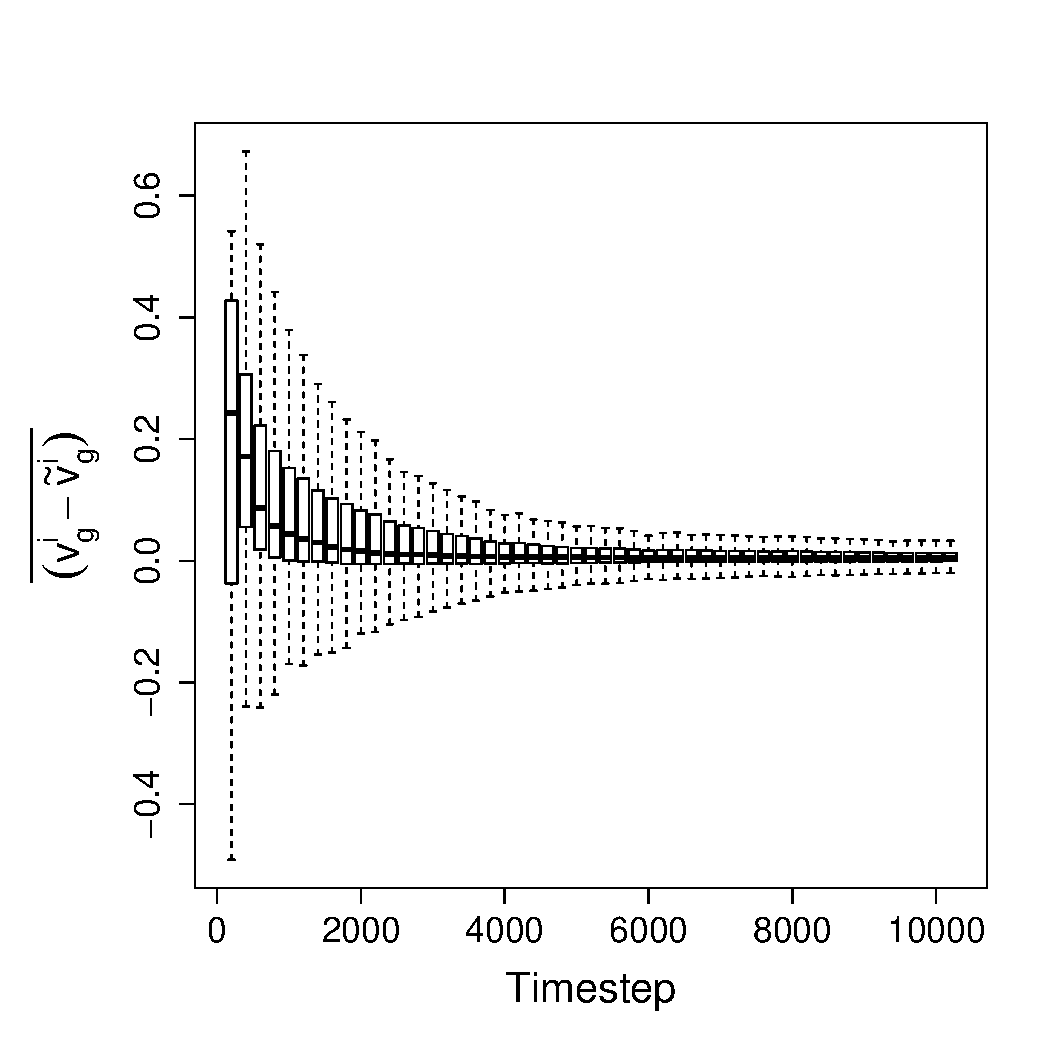
\includegraphics[height=\textwidth]{images/ClearingPriceDistanceEvolutionForTrade-G3N500.pdf}\\
	    \end{columns}
		@~Equilibrium: personal values  $\rightarrow$ optimal (shared) values.
	\end{figure}
	
\end{frame}

\begin{frame}{Results: Frequency Distribution}
    \subsection*{Distribution of variant:}
    \begin{figure}[!h]
	\begin{center}
	    \begin{tabular}{ccc}
		\includegraphics[width=5cm]{../img/2SetupDistribA.pdf}\\
	    \end{tabular}

	\end{center}
	%\caption{Frequencies distribution, where each points represent the mean for 100 runs, for: a) the neutral and the trading models.  b) the neutral model and the trading model without the trading innovation process. c) the trade model and the trade model without the trading innovation process.}
    \end{figure}
\end{frame}

\begin{frame}{Summary}
\begin{itemize}
	\item A local copy mechanism alone is enough to bring the global economy to an optimal equilibrium.
		\vfill
	\item Need a Biased Copy mechanism, Random Copy cannot.
		\vfill
	\item Both mechanisms lead to different frequency distribution.
		\vfill
\end{itemize}

\end{frame}

\section{Application}
\begin{frame}{Case Study}
	Roman Empire Economy: \\
	Tight link between economy and culture, trace of it. \\
	\begin{figure}
		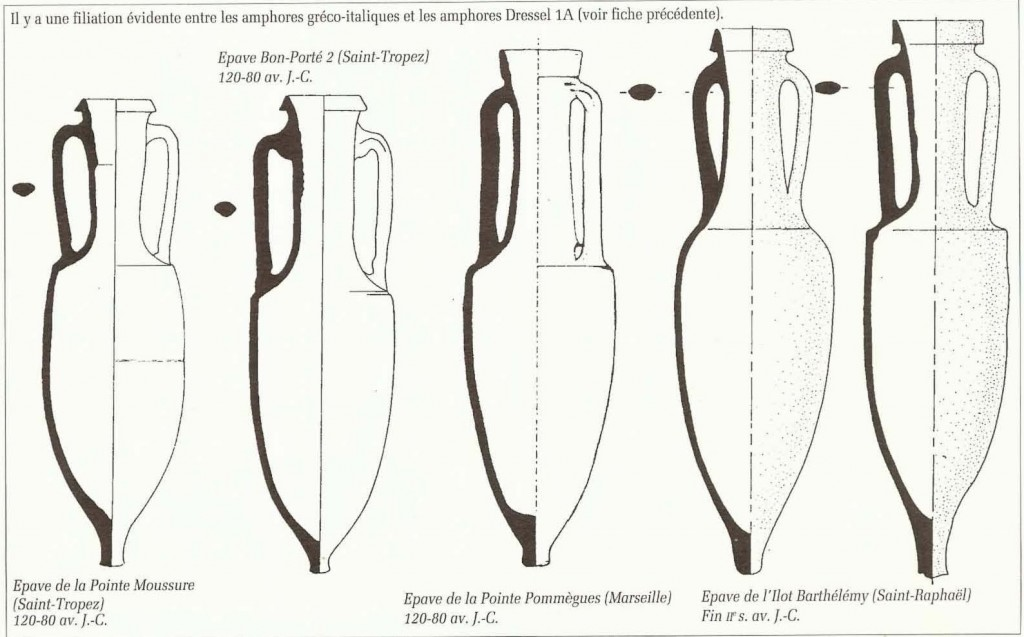
\includegraphics[width=.6\textwidth]{images/dressel-filiation.jpg}
	\end{figure}
	
\end{frame}

\begin{frame}{Case Study}
	Simulation as a tool to implement and test Historical Hypothesis.
	\begin{itemize}
	\item Network Constraints
	\item Temporal Constraints
	\item Different Cultural Mechanisms
	\end{itemize}
\end{frame}
\begin{frame}{Case Study}
	\begin{center}
		\Large
		What was the nature of Roman economy?\\
		
\includegraphics[width=2cm]{images/LOGO-ERC.jpg} \hfil	
\includegraphics[width=3cm]{images/epnetLogo.png}\\
		\vspace{1cm}
		\scriptsize
			http://www.roman-ep.net/\\
			@epnetproject\\
			fb.com/EPNetProject\\
			@simoncarrignon
	\end{center}


\end{frame}

\begin{frame}
    \Huge
    Thank for you attention!
\end{frame}
\end{document}


